\documentclass[12pt,a4paper,notitlepage]{article}

\usepackage[MeX]{polski}
\usepackage[T1]{fontenc}
\usepackage[utf8]{inputenc}
\usepackage[top=3cm, bottom=2cm, left=3cm, right=3cm]{geometry}
\usepackage{graphicx}
  \usepackage{graphics} % wlaczanie grafik
  \usepackage{color}

\makeatletter

    \renewcommand\@seccntformat[1]{\csname the#1\endcsname.\quad}
    \renewcommand\numberline[1]{#1.\hskip0.7em}
\newcommand{\linia}{\rule{\linewidth}{0.4mm}}
\renewcommand{\maketitle}{\begin{titlepage}

    \vspace*{2cm}
\begin{center}\small        
        Instytut Informatyki Uniwersytetu Wrocławskiego\\
        Pracownia Inżynierii Oprogramowania\\
  \vspace{2cm}
        \normalsize \textsc{Grupa 16.}\\
        \normalsize \textsc{\@author}\\
\end{center}
    \vspace{3cm}
    \noindent\linia
    \begin{center}
        \LARGE \textsc{Dokumentacja projektu \textbf{Adminum}}\\       
        \linia
        \vspace{2cm}
        \LARGE \textsc{\@title}\\
      
        \vspace{1.5cm}
       \normalsize \@date\\


    \end{center}
  \end{titlepage}
}
\makeatother

\author{Mirosława Szewczyk, Marek Rybak}
\title{Graficzny interfejs użytkownika}


\begin{document}


    \maketitle
\setcounter{page}{2}
    \tableofcontents
    \newpage
    \section{Interfejs graficzny programu ,,Adminum''}
Na zapotrzebowanie projektu wykonano prototyp programu „Adminum” w skład którego wchodzi również interfejs graficzny, któremu poświęcony jest niniejszy dokument.
Interfejs graficzny programu „Adminum” jest dostępny przy użyciu przeglądarki internetowej. Jest on przystosowany do różnych typów użytkowników, od niezarejestrowanego do administratora, tworząc dla każdego z osobna odmienny rodzaj interfejsu.
   \subsection{Interfejs graficzny dla użytkowników}
W tym podrozdziale zostanie przedstawiony interfejs programu „Adminum” dla niezarejestrowanego gościa serwisu.

Po wejściu do serwisu gość widzi stronę główną, na której znajduje się elektroniczny wniosek rejestracji do sieci. Ponad nim umieszczone jest menu, które pozwala użytkownikowi przemieszczać się między wnioskiem elektronicznym a formularzem zgłaszania usterek. Na stronie głównej jest również możliwość zmiany języka, z domyślnego polskiego na jeden z czterech najpopularniejszych (angielski, niemiecki, francuski, rosyjski), przy pomocy ikonek flag.

W przypadku użytkowników zarejestrowanych lub oczekujących na dodanie do sieci – zamiast wniosku elektronicznego pojawia się ich status w sieci, natomiast na ekranie użytkowników, których prośba o przyłączenie do sieci została odrzucona,  pojawia się informacja z powodem nie zaakceptowania ich wniosku.\\

\scalebox{0.45}{
	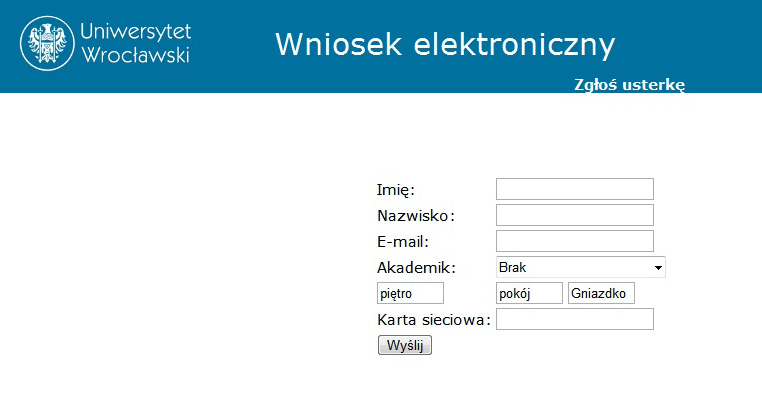
\includegraphics{wniosek.jpg}
}
\begin{center}Rys.1 Strona główna z elektronicznym wnioskiem o przyłączenie do sieci \end{center}



   \subsection{Interfejs graficzny dla administratorów sieci}
Ten podrozdział poświęcony jest interfejsowi graficznemu programu „Adminum” dla administratorów sieci.

Panel administratora jest dostępny po naciśnięciu logo Uniwersytetu Wrocławskiego na stronie głownej – dostępnej dla każdego użytkownika. Administrator zostaje wtedy przeniesiony na stronę logowania, gdzie musi podać swój login i hasło dostępu. Po zalogowaniu do panelu administratora na ekranie widoczne jest menu, z którego można wybrać pomiędzy bazą danych zarejestrowanych użytkowników, listą użytkowników oczekujących na zaakceptowanie przyłączenia do sieci oraz zakładką ze zgłoszonymi usterkami.

Wybierając bazę danych użytkowników, administrator zobaczy tabelę z najważniejszymi informacjami o użytkownikach, tj. imię nazwisko, adres MAC, przydzielone IP, dom studencki oraz nr pokoju. Po kliknięciu na nazwisko wybranego użytkownika, administrator przechodzi do strony z pełnymi danymi podanymi w wniosku elektronicznym, a także może przejrzeć notatki dopisane do użytkownika przez administratorów. W stronie wybranego użytkownika można również ustawić zakres jego możliwości w sieci.

W zakładce dotyczącej użytkowników oczekujących na zaakceptowanie pojawia się lista użytkowników podobna do tej z bazy danych użytkowników, gdzie po kliknięciu i przejściu na stronę użytkownika jest możliwość dodania lub odrzucenia wniosku.

\scalebox{0.45}{
	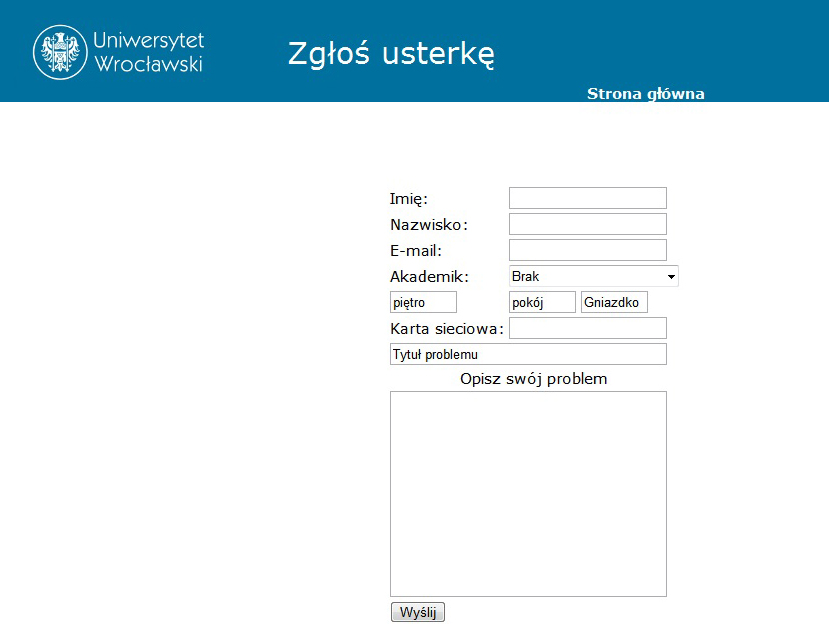
\includegraphics{usterki.jpg}
}
\begin{center}Rys.2 Strona zgłaszania usterek \end{center}

Strona ze zgłoszonymi usterkami przedstawia się w podobny sposób, a mianowicie w postaci listy tematów zgłoszonych usterek oraz numeru pokoju, którego dotyczy. Dopiero po naciśnięciu tematu usterki pojawia się pełen jej opis podany przez użytkownika.












\end{document}